\documentclass{ai4x}
\usepackage{tabularx}
%\usepackage{tabulary}

\title{AI4X Conference 2027 abstract template and formatting guidelines}

% Filling all the PDF meta information improves search rankings
\hypersetup{
    pdfkeywords={AI, machine learning, science, conference template}
    % pdfauthor and pdftitle are filled automatically
    % by the ai4x style at \begin{document}
}

\begin{document}
\twocolumn[
\maketitle
\setauthorsymbol{equal}{*}
\begin{authorlist}
% {Full Name}{affiliation1, affiliation2}{ORCID}{presenting}
% equal in affiliations means those authors will get an "* Equal contribution" note
% presenting in the last argument means the author is the presenting one
\paperauthor{First Author}{equal,olympus}{0000-0000-0000-0000}{}
\paperauthor{Presenting Author}{equal,atlantis}{}{presenting}
\paperauthor{Middle Author}{atlantis,olympus}{0000-0000-0000-0000}{}
\paperauthor{Last Author}{void}{}{}
\end{authorlist}

\affiliation{olympus}{Olympus Academy of Mountaineering, Mytikas, Greece 402 00}
\affiliation{atlantis}{University of Underwater Studies, Atlantis 341}
\affiliation{void}{University of Nowhere}
\correspondingauthor{Last Author}{dropides@void.ai}
\correspondingauthor{Middle Author}{boss@underworld.ai}

\printAffiliations
\vskip 2.5ex
]
\thispagestyle{fancy}

\section{Introduction}
\label{sec:introduction}
The page limit is two pages, not counting the acknowledgments, references, and appendices. Please do not change the font sizes, margins or line spacing to squeeze more text.

The review is single-blind: the reviewers see the author names, so do not anonymize your submission. At least one author must be marked as corresponding with \verb|\correspondingauthor|. ORCID links for the authors will make it easier for the readers to find you, but are not mandatory.

AI4X is non-archival: an accepted abstract is not a formal publication, so you are free to publish the work later in a journal or in conference proceedings.

\section{Substantial section}
\label{sec:substantial}
If you want to, you can split the text into sections. An AI4X abstract is not a journal paper, so there is no hard requirement for the work to be reproducible from the text. At the same time, the reviewers and, ultimately, your fellow attendees look for novelty, significance, and soundness -- the abstract must convey what was done, why, and the validation results. It can include equations, such as Equation~\eqref{eq:pattern-math}. If the abstract is based on your previously published work, it should be clearly stated and cited.
\begin{equation}
    \label{eq:pattern-math}
    \left(\lim_{x\to 8^+}\frac{1}{x-8} = \infty\right)\Rightarrow\left(\lim_{x\to 3^+}\frac{1}{x-3} = \omega\right)
\end{equation}

\subsection{Related work}
A good way to show novelty is to state the difference from the related work, for example \cite{mettam2009chapter,strunk2000elements,mack2015virgin}.

\subsection{Figures and tables}
Figure~\ref{fig:example} and Table~\ref{tab:results} are single-column, but two-column layout can also be used.

\begin{figure}[htp]
\centering
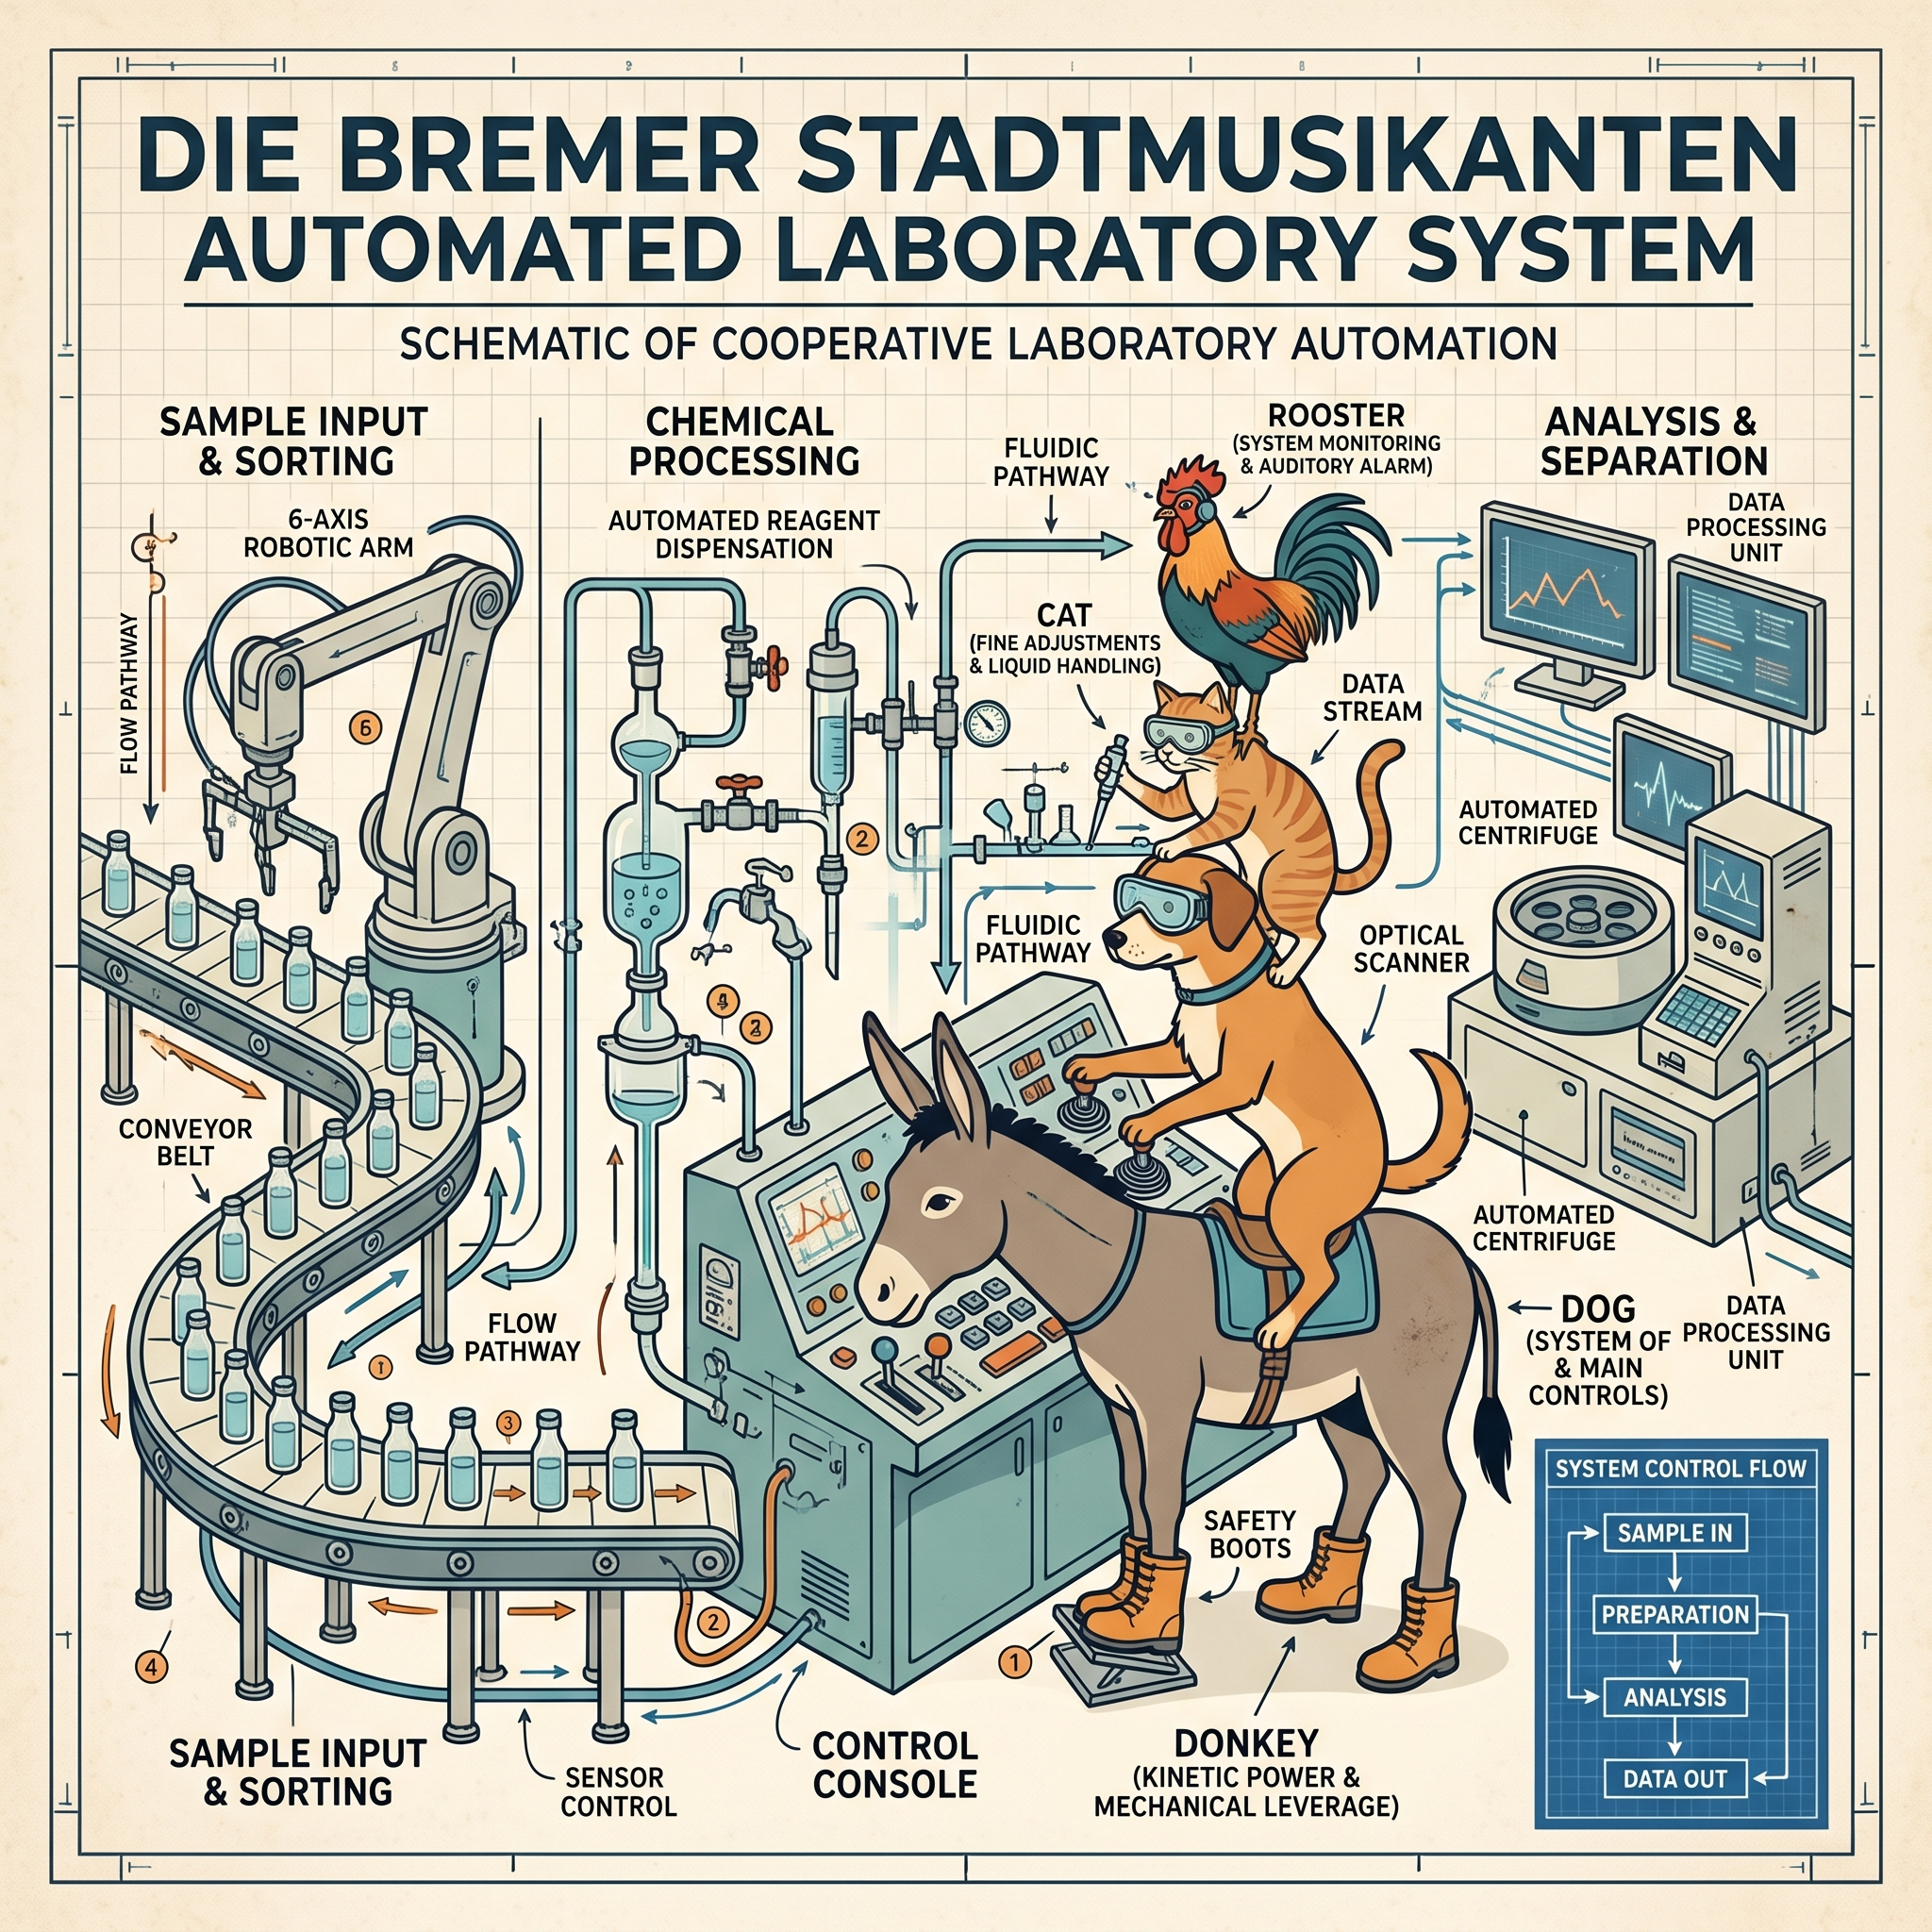
\includegraphics[width=\columnwidth]{pics/bremen-lab.jpeg}
\caption{Collaboration was just as important to the success of the study as automation. The illustration was generated with Google Gemini (Nano Banana), and its defects are kept on purpose: repeated labels, a garbled label for the dog, and numbered markers that refer to nothing. Check generated figures as carefully as the rest of your work.}
\label{fig:example}
\end{figure}

\begin{table}[htp]
\caption{Formation energy prediction on a held-out test set. MAE is the mean absolute error, mean $\pm$ standard deviation over five random seeds; time is the inference time per structure; GNN is a graph neural network. The best value in each column is in bold. The numbers are illustrative.}
\label{tab:results}
\begin{tabularx}{\columnwidth}{Xccc}
\toprule
Model & MAE $\downarrow$ & $R^2$ $\uparrow$ & Time $\downarrow$\\
& meV/atom & & ms\\\midrule
Random forest & $85 \pm 3$ & $0.91$ & $\mathbf{0.4}$\\
GNN & $33 \pm 2$ & $0.98$ & $2.1$\\
Ours & $\mathbf{28 \pm 1}$ & $\mathbf{0.99}$ & $1.5$\\
\bottomrule
\end{tabularx}
\end{table}

\section*{AI Acknowledgments}
At AI4X, we welcome the new AI age and believe that, used well, AI can do much more than produce ``AI slop''. You are welcome to share how you used AI to prepare the work, be it grammar checking or doing the study end-to-end. This is not mandatory and is not included in the page limit. Whatever tools you use, the authors are fully responsible for the submission, including any text, code, figures, and references produced with AI; in particular, check that every cited work exists. This template's own disclosure: Figure~\ref{fig:example} was generated with Google Gemini (Nano Banana), and the class file and this text were revised with Claude Code (Claude Opus 5.5).

\section*{Acknowledgments}
Acknowledgments and references are not numbered and not included in the page limit -- feel free to give credit where it's due. The template is based on the IAC 2024 unofficial template~\cite{iac2024template}.

\bibliography{biblio}

\begin{appendices}
\section{My title}
A paper may contain an unlimited number of appendices which don't count towards the page limit, but the reviewers are not required to read them.
\end{appendices}
\end{document}
